\documentclass[10pt]{article}
\usepackage{icmlko}

\icmlmeta{IP 파운데이션 월드모델}{39}{가르칠 때와 배울 때 다르게 잰다}{노트 38의 상충을 피하는 대신 이용한다 --- 도메인마다 역할별 배선을 두 벌 주면 열둘 중 열하나가 유의해진다}

\begin{document}

\twocolumn[
\icmlheader

\begin{abstract}
노트 38이 상충을 밝혔다 --- 도메인의 인자 공간 자기 상관을 올리면 대상으로서
좋아지고($r=+$0.966) 출처로서 나빠진다($r=-$0.870). 이 노트는 그 상충을 피하는
대신 \textbf{이용한다.} 제품에서 팝업은 대상으로만 쓰므로, 나머지 셋은 자기
라벨을 잘 맞히는 배선이 아니라 팝업으로 잘 옮겨지는 배선을 골라야 한다. 목적
함수가 팝업 라벨을 직접 보므로 선택 편향이 노트 38보다 위험해진다 --- 팝업 75건을
개장 연도로 층화해 탐색용 38건과 확인용 37건으로 나눴다. 탐색 증가는
$+$0.0063인데 확인용 증가는 $+$0.0025로, \textbf{증가분의 60\%가 편향}이었다.
출처별로는 아이돌만 확인용에서도 올랐다($+$0.0600$\to+$0.0694, 15.7\%). 그리고
그 배선이 결정적이다 --- \textbf{노트 38이 자기 상관을 근거로 켠 아이돌 입장
허들(앨범 정가)을, 출처 역할에서는 꺼야 한다.} 같은 축이 역할에 따라 반대
방향이다. 그래서 도메인마다 축을 한 벌이 아니라 두 벌 만들고 셀마다 역할에 맞는
것을 쓰게 했다. \textbf{유의 방향이 10/12에서 11/12로, 평균 이득이 $+$0.0547에서
$+$0.0594로 올랐다}(순열 씨앗 셋에서 동일). 결정적으로, 출처용 배선을 네 도메인에
\emph{일괄} 적용하면 오히려 나빠진다($+$0.0513). 상충이 실재하므로 한 배선으로
두 역할을 다 잘할 수 없다.
\end{abstract}
]

\section{상충을 이용한다}

노트 38의 상충은 나쁜 소식처럼 보였다. 그런데 제품 쪽에서 보면 다르다.

팝업은 \emph{대상으로만} 쓴다. 다른 도메인에서 배워 팝업을 예측하는 것이
목적이고, 팝업으로 남을 가르칠 일이 없다. 그러니 아이돌·게임·도서는 자기 라벨을
잘 맞히는 배선이 아니라 \textbf{팝업으로 잘 옮겨지는 배선}을 고르면 된다.

\paragraph{선택 편향이 더 위험해진다}
노트 38의 목적 함수는 각 도메인의 자기 라벨이었고 팝업 라벨과 무관했다. 이번
목적 함수는 팝업 전이 성적이므로 팝업 라벨을 직접 본다. 후보를 많이 보고
최댓값을 고르면 팝업 라벨에 과적합된다.

그래서 팝업 75건을 개장 연도로 층화해 나눴다 --- 탐색용 38건과 확인용 37건.
연도로 층화하는 것은 시장이 커져 왔기 때문이다(노트 11).

\begin{figure}[t]
\centering

\includegraphics[width=\textwidth]{figs/split.pdf}
\caption{왼쪽 --- 출처별 팝업 이득. 오른쪽 --- 세 출처 평균과 선택 편향.}
\end{figure}

\begin{table}[t]
\centering\tsize
\caption{출처 배선 탐색. 팝업 이득(상수 대비 MAE).}
\begin{tabular}{lrrr}
\toprule
& 탐색용 & 확인용 & 확인 증가 \\
\midrule
현행 & $+$0.0692 & $+$0.0648 & --- \\
승자 & $+$0.0755 & $+$0.0673 & $+$0.0025 \\
\midrule
\multicolumn{4}{l}{선택 편향 $=+$0.0038 (탐색 증가의 60\%)} \\
\bottomrule
\end{tabular}
\end{table}

\begin{table}[t]
\centering\tsize
\caption{출처별. 확인용에서 오른 것은 아이돌뿐이다.}
\begin{tabular}{lrrr}
\toprule
출처 & 현행(확인) & 승자(확인) & 변화 \\
\midrule
\textbf{아이돌} & $+$0.0600 & $+$0.0694 & \textbf{$+$0.0094} \\
게임 & $+$0.0684 & $+$0.0680 & $-$0.0004 \\
도서 & $+$0.0661 & $+$0.0646 & $-$0.0015 \\
\bottomrule
\end{tabular}
\end{table}

\section{같은 축이 역할에 따라 반대다}

탐색이 아이돌에 대해 찾은 것은 둘이다.

\begin{itemize}[leftmargin=1.1em,itemsep=0.15em]
\item \textbf{입장 허들을 끈다} --- 노트 38이 바로 앞에서 켠 것이다.
\item 타깃 폭을 서바이벌 출신으로 --- 데뷔 전 이미 대중에 닿아 있던 정도.
\end{itemize}

\begin{figure}[t]
\centering
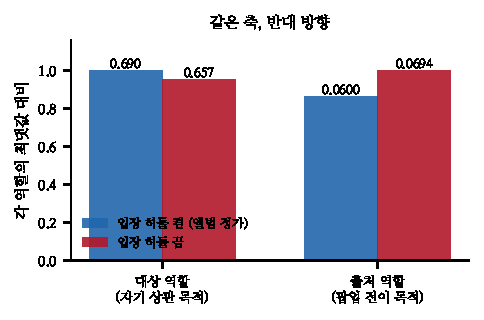
\includegraphics[width=\columnwidth]{figs/faces.pdf}
\caption{아이돌 입장 허들(앨범 정가). 두 역할에서 각각 최댓값 대비로 그렸다.}
\end{figure}

\begin{table}[t]
\centering\tsize
\caption{아이돌 입장 허들 축의 두 얼굴.}
\begin{tabular}{lrr}
\toprule
& 켬(앨범 정가) & 끔 \\
\midrule
대상 역할 (평균 전이 r) & \textbf{$+$0.690} & $+$0.657 \\
출처 역할 (팝업 이득) & $+$0.0600 & \textbf{$+$0.0694} \\
\bottomrule
\end{tabular}
\end{table}

\claimx{같은 축이 같은 도메인에서 역할에 따라 반대 방향으로 작동한다. 아이돌
입장 허들은 켜면 아이돌을 예측하기 쉬워지고 끄면 아이돌이 남을 가르치기
좋아진다.}{다른 축에서도 같은 반전이 나와야 한다. 한 사례뿐이면 아이돌 정가의
특수성일 수 있다.}

\section{그래서 두 벌을 준다}

도메인마다 축을 한 벌이 아니라 두 벌 만들고, 셀 (출처 $s\to$ 대상 $t$)마다
$s$는 출처용, $t$는 대상용을 쓴다.

\begin{figure}[t]
\centering
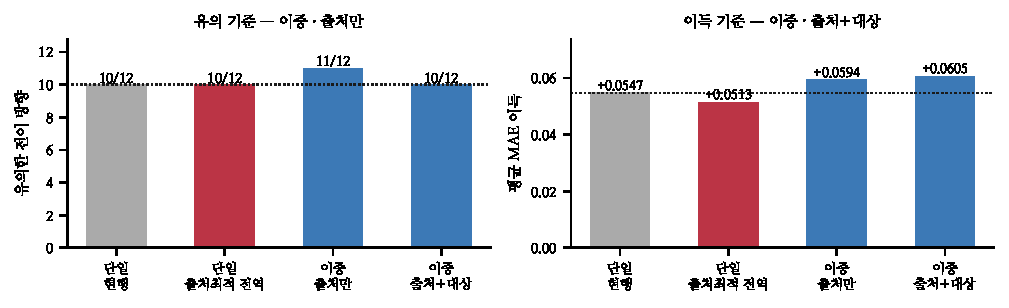
\includegraphics[width=\textwidth]{figs/dual.pdf}
\caption{네 구성. 점선이 현행이다. 순열 씨앗 셋에서 값이 같았다.}
\end{figure}

\begin{table}[t]
\centering\tsize
\caption{배선 구성별 성적. 순열 4000회, 씨앗 셋에서 동일.}
\begin{tabular}{lrr}
\toprule
구성 & 유의 & 평균 이득 \\
\midrule
단일 · 현행 & 10/12 & $+$0.0547 \\
단일 · 출처 최적 전역 & 10/12 & \textbf{$+$0.0513} \\
\textbf{이중 · 출처만} & \textbf{11/12} & \textbf{$+$0.0594} \\
이중 · 출처$+$대상 & 10/12 & $+$0.0605 \\
\bottomrule
\end{tabular}
\end{table}

두 번째 줄이 핵심이다. \textbf{출처용 배선을 네 도메인에 일괄 적용하면 현행보다
나빠진다.} 그 배선이 좋은 것은 출처 역할에서일 뿐이고, 같은 도메인이 대상이
되는 셀에서는 손해다. 상충이 실재하므로 한 배선으로 두 역할을 다 잘할 수 없다.

\begin{table}[t]
\centering\tsize
\caption{바뀐 셀. 나머지 아홉은 그대로다.}
\begin{tabular}{lrrl}
\toprule
셀 & 단일 & 이중 & \\
\midrule
아이돌 $\to$ 팝업 & $-$0.0926 & $-$0.1033 & p 0.014$\to$0.000 \\
아이돌 $\to$ 게임 & $-$0.0042 & $-$0.0232 & \textbf{p 0.289$\to$0.037} \\
아이돌 $\to$ 도서 & $+$0.0064 & $-$0.0168 & p 0.510$\to$0.153 \\
도서 $\to$ 팝업 & $-$0.0877 & $-$0.0888 & \\
도서 $\to$ 아이돌 & $-$0.0745 & $-$0.0753 & \\
도서 $\to$ 게임 & $-$0.0263 & $-$0.0270 & \\
\bottomrule
\end{tabular}
\end{table}

아이돌이 출처인 세 셀이 전부 좋아졌고 그중 하나가 유의로 넘어왔다. 열두 방향 중
남은 하나는 아이돌$\to$도서(p$=$0.153)다.

\claimx{도메인마다 역할별 배선을 두 벌 두면 11/12가 된다. 전역 단일 배선으로는
어느 쪽을 골라도 10/12를 넘지 못한다.}{다섯째 도메인에서 이중 배선의 이득이
사라지면 네 도메인의 우연이다. 특히 아이돌 한 도메인이 이득의 전부이므로
아이돌 특수 현상일 수 있다.}

\section{무엇이 달라졌나}

지금까지 파이프라인은 도메인마다 축을 한 벌 만들었다. 이제 두 벌이다.

\begin{quote}\fontsize{9.5}{11.5}\selectfont
\textbf{출처용} --- 이 도메인이 남을 가르칠 때. 팝업 전이 성적으로 고른다.\\[0.25em]
\textbf{대상용} --- 이 도메인을 예측할 때. 자기 상관으로 고른다(노트 38).
\end{quote}

측정 설계의 관점에서는 자연스럽다. ``무엇을 재느냐''는 ``무엇에 쓰느냐''에
달려 있고, 가르치는 것과 배우는 것은 다른 쓰임이다. 다만 이것은 도메인이
객관적 성질을 갖는다는 그림에서 한 발 물러선 것이기도 하다 --- 축은 이제
용도에 상대적이다.

\paragraph{이득 기준으로는 출처$+$대상이 낫다}
$+$0.0605 대 $+$0.0594다. 그런데 유의는 10/12로 떨어진다. 게임 대상용 배선이
팝업$\to$게임의 이득은 키우면서 다른 셀의 p를 흔든다. 유의 개수를 우선해
출처용만 채택했고, 두 지표가 갈리는 것 자체를 한계로 적는다.

\section{한계}

\begin{itemize}[leftmargin=1.1em,itemsep=0.15em]
\item 이득의 거의 전부가 아이돌 하나에서 나온다. 게임과 도서는 확인용에서
      오히려 미세하게 내려갔다.
\item 팝업 확인용이 37건이다. $+$0.0025의 순증은 이 표본에서 잡음과 구분하기
      어렵다. 열두 셀 순열 검정이 독립 확인 역할을 했지만 그것도 같은 팝업
      데이터를 쓴다.
\item ``출처용/대상용''을 두 벌로 나눴지만 실제로는 출처 역할이 셋(팝업 제외),
      대상 역할이 넷이다. 도메인 쌍마다 다른 배선이 최적일 수도 있고 그러면
      배선 수가 열둘이 된다 --- 그 방향은 과적합이 확실해 보여 시도하지 않았다.
\item 유의 개수와 평균 이득이 갈릴 때 어느 쪽을 따를지 정한 기준이 없다.
\item 아이돌 타깃 폭을 서바이벌 출신(이진)으로 바꿨다. 축의 분산이 0.50으로
      커졌는데 그것이 이득의 원인인지 신호의 질인지 구분하지 않았다.
\end{itemize}

\section{다음}

\begin{enumerate}[leftmargin=1.3em,itemsep=0.15em]
\item 아이돌$\to$도서(p$=$0.153) --- 열둘 중 마지막 하나.
\item 게임과 도서의 출처용 배선을 더 찾는다. 이번 탐색은 후보가 빈약했다.
\item 이진 축의 효과 --- 분산 때문인지 신호 때문인지.
\item 다섯째 도메인 --- 이중 배선의 이득이 아이돌 특수 현상인지 확인한다.
\end{enumerate}

\vspace{0.6em}
\hrule height 0.3pt
\vspace{0.5em}
{\footnotesize
\textbf{참고문헌}\\[0.3em]
Ben-David, S. et al. (2010). A theory of learning from different domains.
\emph{Machine Learning}, 79(1--2), 151--175.\\[0.15em]
Cawley, G. C., Talbot, N. L. C. (2010). On over-fitting in model selection and
subsequent selection bias in performance evaluation. \emph{JMLR}, 11, 2079--2107.\\[0.15em]
Standley, T. et al. (2020). Which tasks should be learned together in multi-task
learning? \emph{ICML}, 9120--9132.\\[0.15em]
Ruder, S. (2017). An overview of multi-task learning in deep neural networks.
\emph{arXiv:1706.05098}.\\[0.15em]
Schönemann, P. H. (1966). A generalized solution of the orthogonal Procrustes
problem. \emph{Psychometrika}, 31(1), 1--10.
}

\end{document}
